\subsection*{Ejercicio 7}

\ejercicio{Implemente un programa que realice la multiplicación de dos
  matrices bidimensionales.  Realice un análisis completo de la
  eficiencia tal y como ha hecho en ejercicios anteriores de este
  guión.}

\begin{flushleft}
  En este ejercicio se ha implementado un programa que utiliza el
  método tradicional para multiplicar matrices y se ha diseñado un
  test donde se expone este programa a la multiplicación de dos
  matrices de iguales dimensiones. El test comienza multiplicando
  matrices de 10x10 con valores aleatorios y realiza en cada test un
  incremento de 10 unidades.
\end{flushleft}

\begin{flushleft}
  A la hora de compilar el código se han generado dos programas con las ordenes siguientes:
\end{flushleft}

\begin{verbatim}
g++ -o prod_opt mult.cpp -O3
g++ -o prod mult.cpp
\end{verbatim}

\begin{flushleft}
  Se ha obtenido la siguiente gráfica que representa los datos obtenidos para ambos tests:
\end{flushleft}

\begin{figure}[H]
  \caption{Multiplicacion de matrices n x n}
  \centering
  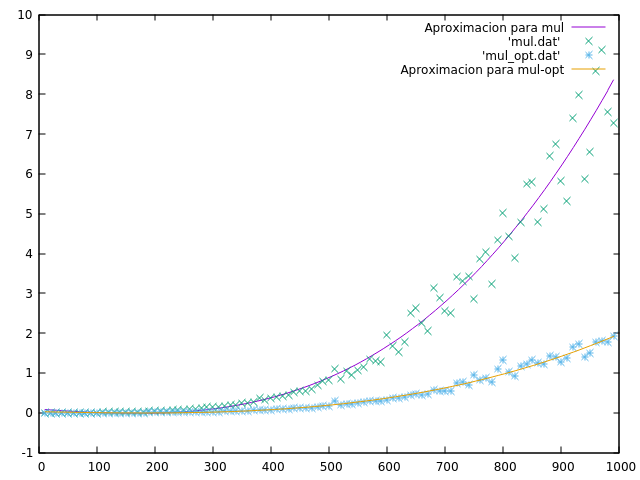
\includegraphics[width=0.8\textwidth]{ejer7/comparacion.png}
\end{figure}

\textbf{Código implementado:} Disponible en la carpeta \textit{ejer7/mult.cpp}